
\documentclass[a4paper,12pt,oneside]{report}

\usepackage{colortbl}

\usepackage{phdthesis}

\usepackage{kostspielig}


\newcommand{\todo}[1]{\textcolor{red}{\textbf{TODO: #1}}}


\title{Design Iteration 3}
\subtitle{Open-source web-app for questionnaires and surveys}
\date{Winter 2011}
\location{University of California Irvine}
\author{Kevin Brotcke\\
Maria Carrasco\\
Andrew Furusawa\\\
Joshua Papa }

\begin{document}
   
\renewcommand{\contentsname}{Contents}
\renewcommand{\bibname}{Bibliography}
\renewcommand{\caption}{{\bf Caption : }}

\raskolnikovmaketitle
\tableofcontents

\chapter{Introduction}

\section{ Purpose}

This document describes the design layout for the Survey Generator program by Team 1000 for their Informatics 117 class during Winter 2011. Major design components such as the data design, architectural and component-level design, and user interface design will be discussed. This is meant as a reference for team members during implementation as well evidence for stakeholders.
\section{ Project Description}

        The project uses a database back-end to generate surveys on-the-fly using a web app. The main components consists of a SQLite database, HTML front-end of surveys and administrator panel, and business logic to generate the surveys.
\chapter{ Data Design}
\section{ Database Description}

        The data will be stored in the form of an embedded SQLite database. (Database scheme outline in progress.)
\section{ Temporary Data Structures}

This will need to import and export XML files in the form XLSX as well as CSV files. These will

only be temporary since they are being converted into and out of the SQLite database.
\chapter{ Architectural and Component-level Design}
\section{ System Structure}
\subsection{ Architecture Diagram}
\begin{figure}[h!]
  \begin{center}
   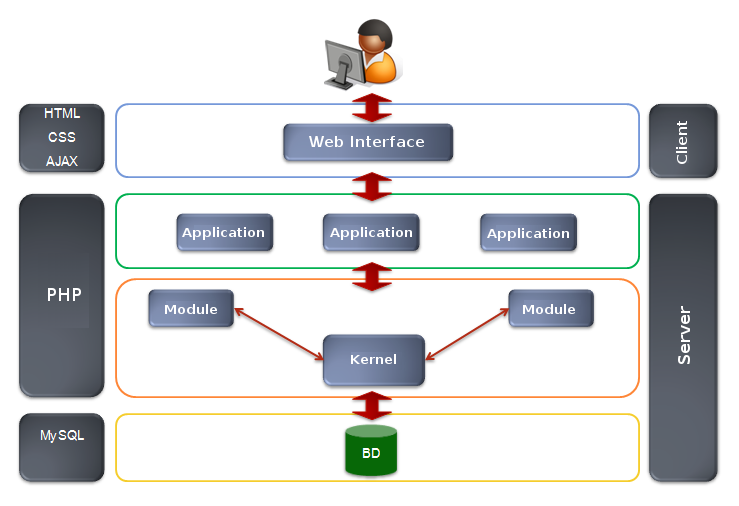
\includegraphics[width=13.5cm]{pics/ar.png}
  \end{center}
\caption{Block Diagram showing major components.}
\end{figure}

\section{Class Diagram}
\begin{figure}[h!]
  \begin{center}
   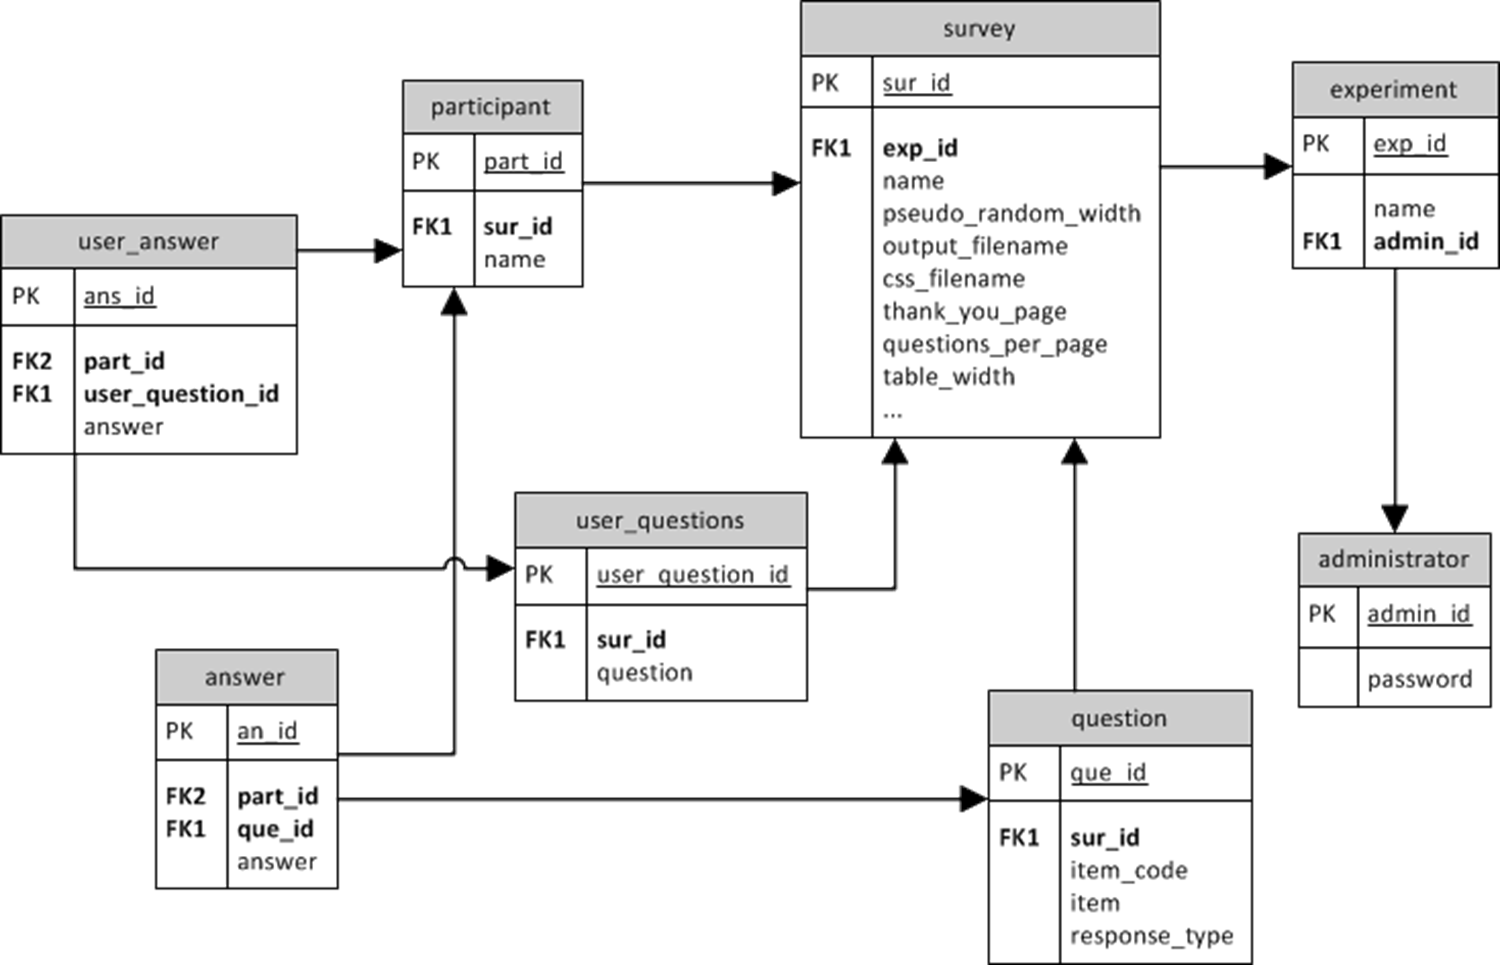
\includegraphics[width=18cm, angle=90]{pics/class.png}
  \end{center}
\caption{Class Diagram.}
\end{figure}

\section{Other Diagrams}
\subsection{Activity Diagrams}
\begin{figure}[h!]
  \begin{center}
   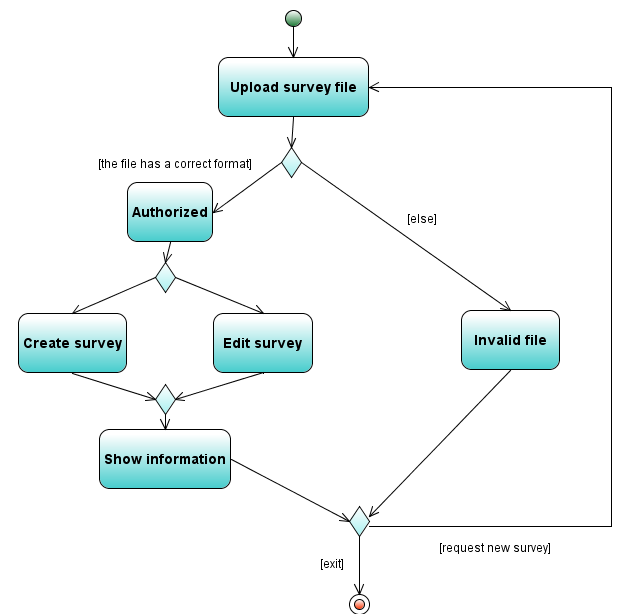
\includegraphics[width=13.5cm]{pics/Activity.png}
  \end{center}
\caption{Activity Diagram for survey creation.}
\end{figure}

\begin{figure}[!hp]
  \begin{center}
   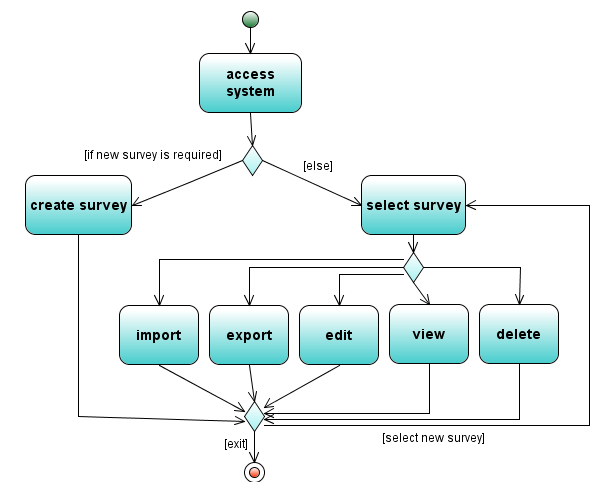
\includegraphics[width=13.8cm]{pics/Activity2.png}
  \end{center}
\caption{Activity Diagram for survey management.}
\end{figure}

\pagebreak

\subsection{Sequence Diagrams}

\begin{figure}[!hp]
  \begin{center}
   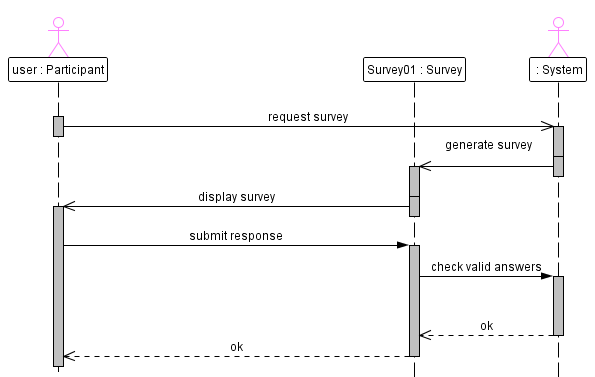
\includegraphics[width=15cm]{pics/Sequence.png}
  \end{center}
\caption{Sequence Diagram.}
\end{figure}

\pagebreak
\subsection{Use Case Diagrams}

\begin{figure}[h!]
  \begin{center}
   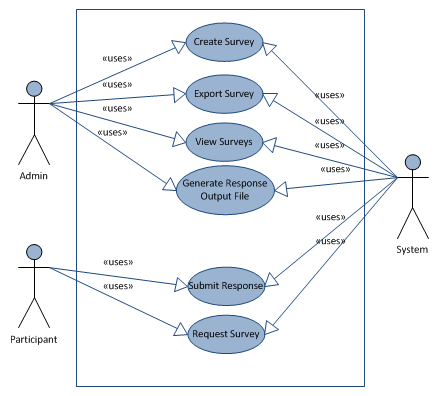
\includegraphics[width=14cm]{pics/usecase.png}
  \end{center}
\caption{Main Use Case Diagram.}
\end{figure}

\chapter{ Restrictions, Limitations, and Contraints}

\section{ Description For Experiment Component}
An experiment will consist in a set of surveys. Each survey should be able to contain three types of inputs:
\begin{description}
\item [text box] It will consists of 0 or more integers.
\item [radio box] Containing one number. It is inclusive.
\item  [yes/no radio box] Allowing a two choice answer.
\end{description}
The system will support infinite surveys and experiments.

\section{ Description For User Component}

The user or participant shall be able to perform the following actions:
\begin{itemize}
	\item Request Survey by URL \\ Correct survey automatically assigned to user based off URL.
	\item Submit Survey Response
\end{itemize}
\section{  Description For Administrator Component}

Although our design will allow the possibility of future additions of administers easily, initially we will only have one. The administrator shall be able to do the following actions:
\begin{itemize}
	\item Create Survey \\ transfer a new xlsx file via ftp to an input folder
	\item Edit Survey \\ overrides the existing xlsx file
	\item View Survey \\ downloads the xlsx file from the server
	\item Download Results 
\end{itemize}

\section{Description for the Output File}
The exported results will be in {\bf csv} format. The mush contain the following restrictions:
\begin {itemize}
\item Additional column for survey title.
 \item Do not have to support excel.
\end{itemize}


\chapter{ User Interface Design}

\section{  Description Of The User Interface}

The main features that the software will present are:
\begin{itemize}
\item {\it Sets of surveys}, allowing the user to automatically loop through them.
\item {\it Pseudo-Randomization} of the order of the surveys.
\item {\it Result file}. This file will contain these main fields: Subject ID, survey number, code and responses.
\end{itemize}

\subsubsection { Appearance Of Surveys}
\begin{itemize} 
	\item  the appearance of the sentences on the web form (font, size, color, spacing, location, etc) needs to be customizable through CSS/HTML tags
	\item the web form needs to accept a couple of different response types (radio buttons, text boxes, etc)
	\item Left/Center/Right justifiable
	\item autocomplete off
	\item css template file option
	\item sentences per page
\end{itemize}

\subsection{ Screen Images}
\subsection{ Objects And Actions}



\end{document}
